\documentclass[12pt,oneside,a4paper]{book} % This style for A4 format.

%Packages
\usepackage{ecproject}
\usepackage{graphicx}
\usepackage{tikz}
\usetikzlibrary{calc}
\usepackage[a4paper, margin=1in]{geometry}
\usepackage{float}
\usepackage{qrcode}
%%%Page related
\usepackage{fancyhdr} % for header & footer
\usepackage[hidelinks]{hyperref}
\usepackage[toc, nonumberlist]{glossaries} %For Glossaries - to be loaded only after hyperref package
%\ifIndentPara
\usepackage{indentfirst}
%\fi
\usepackage{setspace}
%%%Table Related
%\usepackage{booktabs}
%\usepackage{makecell}
%\usepackage{multirow}
%\usepackage{multicol}


%Document settings
\title{Design and Analysis of Oversampling ADC}
%%%%%%%%%%%%%%%Minor (or) Major report%%%%%%%%%%%%%%%
%Uncomment \MinorProject line, if the report is for Minor project.
\MinorProject
%%%%%%%%%%%%%%%%%%%%%%%%%%%%%%%%%%%%%%%%%%%%%%
%%%Student Details%%%
\stuNameA{Sahana K S}
\stuUSNA{1RV17EC190}
\stuNameB{Rakshata Karlingannavar}
\stuUSNB{1RV17EC119}
\stuNameC{Roshni Sen}
\stuUSNC{1RV16EC007}
%\stuNameD{Subrahmanya K N}
%\stuUSND{1RV16EC007}

%%%Internal Guide%%%%
\guideNameA{Mr. Subrahmanya K N}
\guideDesignationA{Assistant Professor}
\guideDeptA{Dept. of ECE}
\guideOrgA{RV College of Engineering}

%%%External Guide%%%%
%\guideNameB{Dr. Ramavenkateshwaran}
%\guideDesignationB{Assistant Professor}
%\guideDeptB{Dept. of ECE}
%\guideOrgB{RV College of Engineering}

%\guideNameC{Dr. Ramavenkateshwaran}
%\guideDesignationC{Assistant Professor}
%\guideDeptC{Dept. of ECE}
%\guideOrgC{RV College of Engineering}

\panelMemberA{Dr. Kariyappa}
\panelMemberDesigA{Professor}
\panelMemberB{Dr. Ramavenkateshwaran}
\panelMemberDesigB{Assistant Professor}

\Department[ECE]{Electronics and Communication Engineering}

\HOD{Dr. K S Geetha}
\Principal{Dr. K. N. Subramanya}

\academicYear{2020-2021}

\QRurl{}
%\QRurl{https://drive.google.com/open?id=1jm-POmuq-ZZ1tT5m-xAdCDRnwvLZH8q-}
%%%%%%%%%%%%%%%%%%%For PG program%%%%%%%%%%%%%%%%%%%
%%%Uncomment \pgProgram command and define appropriate values for \MastersIn{} and \pgProgramName{}

%\pgProgram%
\MastersIn[M.Tech]{Master of Technology}
\pgProgramName{VLSI Design \& Embedded Systems}

%%%%%%%%%%%%%%%%%%Draft report%%%%%%%%%%%%%%%%%%
\DraftCopy
%%%%%%%%%%%%%%%%%%%%%%%%%%%%%%%%%%%%%%%%%%%%%%

%%%%%%%%%%%%%%%%%%Acronyms%%%%%%%%%%%%%%%%%%
\newglossary[sym]{symbolList}{sym1}{sym2}{List of Symbols}
\makeglossaries
%Acronyms
\loadglsentries{./AuxFiles/Glossaries}
\renewcommand{\glspostdescription}{}% To remove dot at the end
%%%%%%%%%%%%%%%%%%%%%%%%%%%%%%%%%%%%%%%%%%%%%%

%%%%%%%%%%%%%%Bibliography%%%%%%%%%%%%%%%%%%%%%
\usepackage[backend=biber,style=ieee]{biblatex}
%If backend is set to bibtex, then configure texmaker Bi(La)Tex with "bibtex %"
\addbibresource{./AuxFiles/ProjectBib.bib}%Add bib file with extention
%%%%%%%%%%%%%%%%%%%%%%%%%%%%%%%%%%%%%%%%%%%%%%

%%%%%%%%%%%%%%%%WaterMark%%%%%%%%%%%%%%%%%%%%%
%%Use it only after Biblatex
\usepackage[printwatermark]{xwatermark}
\newwatermark[allpages,color=gray!50,angle=0,scale=2,xpos=0,ypos=0]{
\includegraphics[width=0.3\textwidth]{Figures/RVlogoVecW}}
%\usepackage{background}
%\backgroundsetup{scale=1, angle=0, firstpage = true, opacity=1, contents={
%\begin{tikzpicture}[remember picture, overlay]
%\node at ([yshift=0pt, xshift=0pt]current page.center){\includegraphics[width=0.3\textwidth]{Figures/RV_logoVecW}};
%\end{tikzpicture}
%}}
%%%%%%%%%%%%%%%%%%%%%%%%%%%%%%%%%%%%%%%%%%%%%%
\begin{document}
\maketitle
%\pagestyle{empty}
\newpage
\begin{spacing}{1.5}
%%ecproject package is created by P Narashimaraja, Assistant Professor, ECE, RVCE
%Border
\begin{tikzpicture}[remember picture, overlay]
  \draw[line width = 4pt] ($(current page.north west) + (0.75in,-0.75in)$) rectangle ($(current page.south east) + (-0.75in,0.75in)$);
\end{tikzpicture}
\thispagestyle{empty}
\vspace{-1cm}
\begin{center}
\Large\textbf{RV College of Engineering\textsuperscript{\small\textregistered}, Bengaluru} \par
\large{(\textit{Autonomous institution affiliated to VTU, Belagavi})} \par
\large\textbf{Department of \printDepartmentLF}\\
.\hspace{2cm}\\

\includegraphics[width=4cm]{Figures/RV_logoVec}\par
\Large\textbf{\underline{CERTIFICATE}} \par
\end{center}
%\begin{minipage}[b]{\linewidth}
%\large
\begin{spacing}{1.5}
\noindent Certified that the \ifMinor{minor\;}\else{ major\;}\fi project work titled \textbf{\textit{\printTitle}} is carried out by
\ifPG{%
\textbf{\printStuNameA} (\textbf{\printStuUSNA}) who is  bonafide student 
}
\else{
\ifStuNameDUsed{%
\textbf{\printStuNameA } (\textbf{\printStuUSNA}), \textbf{\printStuNameB } (\textbf{\printStuUSNB}), \textbf{\printStuNameC } (\textbf{\printStuUSNC}) and \textbf{\printStuNameD } (\textbf{\printStuUSND})  who are bonafide students 
}\else{% 
\ifStuNameCUsed{%
\textbf{\printStuNameA } (\textbf{\printStuUSNA}), \textbf{\printStuNameB } (\textbf{\printStuUSNB}) and \textbf{\printStuNameC } (\textbf{\printStuUSNC})  who are bonafide students 
}\else{%
\ifStuNameBUsed{%
\textbf{\printStuNameA} (\textbf{\printStuUSNA}) and \textbf{\printStuNameB} (\textbf{\printStuUSNB})  who are bonafide students 
}\else{%
\textbf{\printStuNameA} (\textbf{\printStuUSNA}) who is  bonafide student 
}
\fi
}\fi
}\fi
}\fi
of RV College of Engineering, Bengaluru, in partial fulfillment of the requirements for the degree of  \ifPG \textbf{\printMastersInLF} in \textbf{\printMastersPrgName} \else\textbf{Bachelor of Engineering} in \textbf{\printDepartmentLF} \fi of the Visvesvaraya Technological University, Belagavi during the year \printAcadYear. It is certified that all corrections/suggestions indicated for the Internal Assessment have been incorporated in the \ifMinor{minor\;}\else{major\;}\fi project report deposited in the departmental library. The \ifMinor{minor\;}\else{ major\;}\fi project report has been approved as it satisfies the academic requirements in respect of \ifMinor{minor\;}\else{ major\;}\fi project work prescribed by the institution for the said degree.\\ \par
\end{spacing}

\begin{table}[H]
\centering
\resizebox{1\textwidth}{!}{%
\begin{tabular}{ccc}
\large Signature of Guide &\large Signature of Head of the Department &\large Signature of Principal\\
& &\\
\large\printGuideNameA & \large\printHOD & \large\printPrincipal\\
& & \\
\end{tabular}%
}
\end{table}

\begin{table}[H]
\centering
%\resizebox{\textwidth}{!}{%
\begin{tabular}{lccp{6cm}cc}
&&&\textbf{External Viva}&&\\
&&&&&\\
&Name of Examiners &&& & Signature with Date\\
&&&&&\\
1.&&&&&\\
&&&&&\\
2.&&&&&\\
\end{tabular}%
%}
\end{table}
%\pagebreak
\newpage
%%ecproject package is created by P Narashimaraja, Assistant Professor, ECE, RVCE
%%Border
\begin{tikzpicture}[remember picture, overlay]
  \draw[line width = 4pt] ($(current page.north west) + (0.75in,-0.75in)$) rectangle ($(current page.south east) + (-0.75in,0.75in)$);
\end{tikzpicture}

\thispagestyle{empty}

\begin{center}
\Large\textbf{\underline{DECLARATION}} \par
\end{center}


\noindent \ifPG I \else \ifStuNameBUsed We\else I\fi\fi, \textbf{\printStuNameA} \ifPG \else\ifStuNameBUsed  \ifStuNameCUsed ,$\,$ \else{$\,$ and $\,$}\fi \textbf{\printStuNameB} \ifStuNameCUsed  \ifStuNameDUsed ,$\,$ \else{$\,$ and $\,$}\fi \textbf{\printStuNameC}$\,$ \ifStuNameDUsed and $\,$ \textbf{\printStuNameD}$\,$ \fi \fi \fi \fi students of \ifPG fourth \else \ifMinor{seventh\;}\else{eighth\;}\fi \fi semester \ifPG \printMastersInSF\, in \printMastersPrgName \else B.E.\fi, Department of \printDepartmentLF, RV College of Engineering, Bengaluru, hereby declare that the \ifMinor{minor\;}\else{ major\;}\fi project titled `\textbf{\printTitle}' has been carried out by \ifStuNameBUsed us \else me \fi and submitted in partial fulfilment for the award of degree of \ifPG \textbf{\printMastersInLF} in \textbf{\printMastersPrgName} \else\textbf{Bachelor of Engineering} in \textbf{\printDepartmentLF} \fi during the year \printAcadYear.\\ \par

\noindent Further \ifPG I \else\ifStuNameBUsed we \else I \fi \fi declare that the content of the dissertation has not been submitted previously by anybody for the award of any degree or diploma to any other university.\\ \par

\noindent \ifPG I \else\ifStuNameBUsed We \else I \fi \fi also declare that any Intellectual Property Rights generated out of this project carried out at RVCE will be the property of RV College of Engineering, Bengaluru and we will be one of the authors of the same.

\vspace{1cm}
\noindent Place: Bengaluru\par
\vspace{0.5cm}
\noindent Date: \par

\vspace{2cm}
\begin{table}[H]
\centering
%\resizebox{\textwidth}{!}{%
\begin{tabular}{llcp{5cm}cc}
&&&&&\\
&&&&&\\
&Name  &&& Signature& \\
&&&&&\\
1.&\printStuNameA (\printStuUSNA)&&&&\\
&&&&&\\
\ifPG% 
\else%
\ifStuNameBUsed%
2.&\printStuNameB (\printStuUSNB)&&&&\\
&&&&&\\
\else%
\fi%
\ifStuNameCUsed%
3.&\printStuNameC (\printStuUSNC)&&&&\\
&&&&&\\
\else%
\fi%
\fi%
\end{tabular}%
%}
\end{table}
%\pagebreak


\newpage
%%ecproject package is created by P Narashimaraja, Assistant Professor, ECE, RVCE.
%%Border
\begin{tikzpicture}[remember picture, overlay]
  \draw[line width = 4pt] ($(current page.north west) + (0.75in,-0.75in)$) rectangle ($(current page.south east) + (-0.75in,0.75in)$);
\end{tikzpicture}
\thispagestyle{empty}

\begin{center}
%.\hspace{1cm}\\ \par
\Large\textbf{\underline{ACKNOWLEDGEMENT}} \par
\end{center}

\ifPG I am \else
\ifStuNameBUsed We are \else I am \fi\fi indebted to \ifPG my \else\ifStuNameBUsed our \else my \fi\fi guide, \textbf{\printGuideNameA}, \printGuideDesigA, \printGuideOrgA$\,.$ for the wholehearted support, suggestions and invaluable advice throughout \ifPG my \else\ifStuNameBUsed our \else my \fi\fi project work and also helped in the preparation of this thesis.\\ \par

\ifPG I \else \ifStuNameBUsed We \else I \fi\fi also express our gratitude to \ifPG my \else\ifStuNameBUsed our \else my \fi\fi  panel members \textbf{\printPanelMemberA}, \printPanelMemberDesigA $\,$ and \textbf{\printPanelMemberB}, \printPanelMemberDesigB , Department of \printDepartmentLF\, for their valuable comments and suggestions during the phase evaluations. \\ \par

\ifPG My \else \ifStuNameBUsed Our \else My \fi\fi sincere thanks to \textbf{\printHOD}, Professor and Head, Department of \printDepartmentLF, RVCE for the support and encouragement.\\ \par

\ifPG I \else \ifStuNameBUsed We \else I \fi\fi express sincere gratitude to our beloved Principal, \textbf{\printPrincipal} for the appreciation towards this project work.\\ \par

\ifPG I \else\ifStuNameBUsed We \else I \fi\fi thank all the teaching staff and technical staff of \printDepartmentLF\, department, RVCE for their help.\\ \par 

Lastly, \ifPG I \else\ifStuNameBUsed we \else I \fi\fi take this opportunity to thank \ifPG my \else\ifStuNameBUsed our \else my \fi\fi family members and friends who provided all the backup support throughout the project work.\\ \par

%\pagebreak
\newpage
\pagenumbering{roman}
\chapter*{Abstract}
\addcontentsline{toc}{chapter}{Abstract}\vspace{-1cm}
%Border
\begin{tikzpicture}[remember picture, overlay]
  \draw[line width = 4pt] ($(current page.north west) + (0.75in,-0.75in)$) rectangle ($(current page.south east) + (-0.75in,0.75in)$);
\end{tikzpicture}


% Highlights of significant contributions: One page with 3 to 4 paragraphs\\

% Paragraph 1: Importance of Topic, Present shortcomings in performance or computation etc, issues involved in the shortcomings, short on what is done in this report addressing shortcomings

Technology is an evolutionary process that has gained traction in business, academia and government in the recent years. Lectures in classrooms have advanced to the extent of using smart-boards and smart-classrooms. However, there exists an absence of any technological advancement regarding jotting down notes during a presentation or seminar. Our project aims to aid the attendees of any seminar, presentation or lecture in recording vital information in the form of concise notes. The main shortcoming was lack of GPU and limited RAM availability. Due to this, denoising autoencoder had to be trained on very few images. This might make the model vulnerable to overfitting, hence leading to model memorising the training images and producing very high training accuracy and very low validation accuracy. This was avoided by using L2 regularization which avoids overfitting of the model by penalising the weights that are very large.\\

% Paragraph 2 Objectives of this work, short on algebraic methods used and formulations achieved, computational procedures developed. 

The objectives of our project were to develop and train a denoising autoencoder to deblur the input image, to build an object detection model to detect text from the deblurred image and finally, to extract the detected text and summarize it using extractive summarization. By doing so, we will achieve the goal of our visual summarizer, that is to generate concise notes from any presentation or lecture.\\


% Paragraph 3: Description of simulation procedure including SW tools used and choice of test cases. Short on results achieved and significant highlights of improvements if any.

The software tools used for our project include PyCharm, Google Colab and LabelImg. Software libraries used to train machine learning models are Tensorflow, Keras, \acrshort{ocv}, PyTesseract, NLTK (Natural Language Processing Toolkit), matplotlib, pandas and numpy to name a few. We have achieved a very efficient reconstruction of blurred images and, successfully implemented text extraction and summarization on them. Model accuracies can be further improved by increasing the size of the image dataset and training for more number of epochs.

\pagebreak
\end{spacing}
\newpage
\pagestyle{fplain}
\begin{spacing}{1.5}
	\tableofcontents	
\end{spacing}
\newpage
\begin{spacing}{1.5}
	\cleardoublepage
	\addcontentsline{toc}{chapter}{\listfigurename}
	\listoffigures	
\end{spacing}
\newpage
\begin{spacing}{1.5}
	\cleardoublepage
	\addcontentsline{toc}{chapter}{\listtablename}
	\listoftables	
\end{spacing}
\newpage
\printglossary[type=\acronymtype, title= Abbreviations, toctitle=Abbreviations]
\newpage
\printglossary[type=symbolList, title= List of Symbols, toctitle=List of Symbols]

\mainmatter
\pagestyle{mplain}
\glsresetall
\begin{spacing}{1.5}
%Chapter 1 
\chapter{Introduction to Analog and Digital converters}
Every chapter should start with an introduction paragraph. This paragraph should brief about the flow of the chapter. This introduction can be limited within 4 to 5 sentences. The chapter heading should be appropriately modified (a sample heading is shown for this chapter).
\section[Introduction]{\textbf{Introduction}}
The title of the project can be introduced in this section. This section should neatly elaborate the context of the project, the relevance of the area chosen and the title. You can bring a brief history and arrive at the title of the project. Use appropriate number of paragraphs within this section. 

You are allowed to use figures or diagrams which can help in introducing the topic acknowledging the source. For example , if you are introducing a particular topic, an appropriate figure can be used. The figure should be referenced in the text as Figure. \ref{fig:universe} 
\begin{figure}[htb]
\centering
	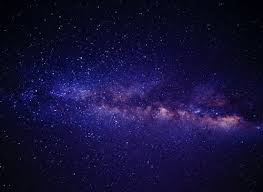
\includegraphics[scale=1]{Figures/universe}	
	\caption{Sample picture of universe }
	\label{fig:universe}
\end{figure}

These guidelines are provided to formally expose you to the various ethical and technical issues involved in writing up your work and the format you are required to adhere to while submitting your project report.

\section[Motivation]{\textbf{Motivation}}

Brief the motivation of selecting your project title. You can elaborate the challenges in the specific area, relevance and importance of the chosen topic. 

\section[Problem statement]{\textbf{Problem statement}}

Define the problem statement in this section, in one paragraph.

\section[Objectives]{\textbf{Objectives}}
The objectives of the project are
\begin{enumerate}
\item To design a pipelined ADC for audio frequency range
\item List all the objectives in the above format , starting with "To"
\item Limit the number of objectives to a maximum of three
\end{enumerate}

\section[Literature Review]{\textbf{Literature Review}}

A literature review is a text of a scholarly paper, which includes the current knowledge including substantive findings, as well as theoretical and methodological contributions to a particular topic. Literature reviews are secondary sources, and do not report new or original experimental work. Most often associated with academic-oriented literature, such reviews are found in academic journals, and are not to be confused with book reviews that may also appear in the same publication. Literature reviews are a basis for research in nearly every academic field . A narrow-scope literature review may be included as part of a peer-reviewed journal article presenting new research, serving to situate the current study within the body of the relevant literature and to provide context for the reader. In such a case, the review usually precedes the methodology and results sections of the work.

\subsection{Sample}
The main types of literature reviews are: evaluative, exploratory, and instrumental. A fourth type, the systematic review, is often classified separately, but is essentially a literature review focused on a research question, trying to identify, appraise, select and synthesize all high-quality research evidence and arguments relevant to that question. A meta-analysis is typically a systematic review using statistical methods to effectively combine the data used on all selected studies to produce a more reliable result.
\subsubsection[Review types]{\textbf{Review types}}

The main types of literature reviews are: evaluative, exploratory, and instrumental. A fourth type, the systematic review, is often classified separately, but is essentially a literature review focused on a research question, trying to identify, appraise, select and synthesize all high-quality research evidence and arguments relevant to that question. A meta-analysis is typically a systematic review using statistical methods to effectively combine the data used on all selected studies to produce a more reliable result.


\subsubsection[Process and product]{\textbf{Process and product}}

Distinguish between the process of reviewing the literature and a finished work or product known as a literature review. The process of reviewing the literature is often ongoing and informs many aspects of the empirical research project. All of the latest literature should inform a research project. Scholars need to be scanning the literature long after a formal literature review product appears to be completed.

\subsubsection{\textbf{Page limitation}}

A careful literature review is usually 15 to 30 pages and could be longer. The process of reviewing the literature requires different kinds of activities and ways of thinking and link the activities of doing a literature review with Benjamin Bloom’s revised taxonomy of the cognitive domain (ways of thinking: remembering, understanding, applying, analysing, evaluating, and creating).

This section should contain the review of the literature in the past.You should review a minimum of 10 papers from standard reference journals. Kindly avoid local conference papers and papers from predatory journals. Kindly consult with your guide and finalize papers to be considered for review before adding in this section.Report the major observations and findings from each paper in one paragraph in the format given below.

 proposed various techniques for adders and multipliers.Add the reference papers to the bibliography section using Jabref and cite it here using the instructions given in further chapters.


\subsubsection{\textbf{Plagiarism}}

To use someone else's exact words without quotation marks and appropriate credit, or to use the unique ideas of someone else without acknowledgement, is known as plagiarism. In publishing, plagiarism is illegal; in other circumstances, it is, at the least, unethical. You may quote or paraphrase the words or ideas of another if you document your source. Although you need not enclose the paraphrased material in quotation marks, you must document the source. 

Paraphrased ideas are taken from someone else whether or not the words are identical. Paraphrasing a passage without citing the source is permissible only when the information paraphrased is common knowledge in a field. (Common knowledge refers to historical, scientific, geographical, technical, and other type of information on a topic readily available in handbooks, manuals, atlases and other references). 

\subsubsection{How to add Reference}
Use \texttt{Jabref} which will help in adding the reference in a separate file, from which one can use \verb|\citep\{\}| command to add reference. A sample, referring to a textbook would look something like this,\cite{Razavi2000}.

\section[Brief Methodology of the project]{\textbf{Brief Methodology of the project}}
Discuss about the methodology you identified to execute the objectives of your project in brief. Methodology is a system of practices, techniques, procedures, and rules used to execute a particular project. You can elaborate the methodology in a later chapter. Here you can present in the form of a flow diagram and explain the methodology in a paragraph.

\section[Assumptions made / Constraints of the project]{\textbf{Assumptions made / Constraints of the project}}

List the assumptions made for the execution of the project in this section. You can also elaborate on the major constraints of the project. This section should clearly state under what conditions your project is valid. It is mandatory to have this section in your project report.

\section[Organization of the report]{\textbf{Organization of the report}}

This report is organized as follows. Write the discussions in each chapter. A sample is as follows.
\begin{itemize}
\item Chapter 2 discusses the fundamentals of ADC and the performance parameters for evaluation.
\end{itemize}

In a similar way, write briefly about each chapter in one or two sentences.

%Chapter 2
\chapter{Convolutional Neural Networks (CNN)}

In Convolutional Neural Networks, the goal is to provide an image as an input and generate an output that determines the probability of the image belonging to a certain class. This chapter discusses the fundamentals of CNN as well as its various layers, i.e the Convolutional Layer, the Pooling Layer and the Fully Connected Layer.
\section{Introduction to \acrlong{cnn}}

Artificial Intelligence has contributed in a monumental manner to bridge the gap between humans and computer abilities. To make great things possible, researchers work on various facets of the area, the domain of Computer Vision being one of several such fields. The goal for this field is to allow machines to view the world as humans do, interpret it in a similar way and even use information for a variety of tasks, such as recognition of images and videos, reconstruction of media, recommendation systems, processing of natural languages, and so on. With time, the advances in Computer Vision with Deep Learning have been developed and refined, predominantly through a specific algorithm, a Convolutional Neural Network.

A Convolutional Neural Network (ConvNet/\acrshort{cnn}) is a deep learning algorithm that can take an input image, assign significance to various aspects/objects in the image and be able to distinguish one from the other. In comparison to other classification algorithms, the pre--processing required in a CNN is much lower. In \acrshort{cnn}, filters are not hand-engineered -- with enough training, they have the ability to learn these filters. 

The architecture of Convolutional Neural Networks differs from that of regular Neural Networks. In case of regular Neural Networks, an  is transformed by passing it through multiple hidden layers where each layer consists of a set of neurons and is entirely connected to all neurons in the layer before, following which there is a final fully-connected layer — the output layer — that represents the predictions. There is a slight difference in case of Convolutional Neural Networks. Here, the layers are organised in 3 dimensions: width, height and depth. Further, the neurons in one layer do not connect to all the neurons in the next layer but only to a small region of it. Ultimately, the final output will be reduced to a single vector of probability scores, organized along the depth dimension.
\section{Working of \acrlong{cnn}}
A \acrshort{cnn} has several layers for processing an image which are discussed below.
\subsection{Convolution Layer}
This is the first layer to extract features from an input image. An image is nothing but a matrix of pixel values. Convolution preserves the relationship between pixels by learning image features using small squares of input data. It is a mathematical operation that takes two inputs such as image matrix and a filter or kernel to produce a feature map. Convolution is executed by sliding the filter over the input. At every location, a matrix multiplication is performed between the image matrix and the filter matrix and the result is summed onto the feature map as shown in figures \ref{fig:imagemat} and \ref{fig:outputmat}. 

% \ref{fig:object} 
\begin{figure}[H]
\centering
	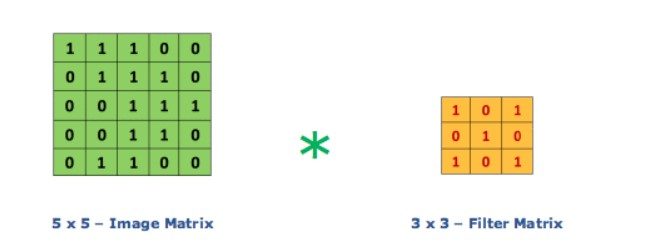
\includegraphics[scale=1]{Chapter2/img_mat_mul_kernel_filter_matrix.jpg}	
	\caption{Image matrix multiplied with kernel or filter matrix}
	\label{fig:imagemat}
\end{figure}
\begin{figure}[H]
\centering
	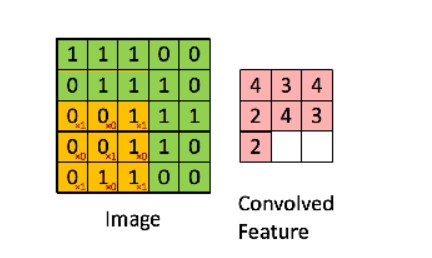
\includegraphics[scale=1]{Chapter2/output_mat.jpg}	
	\caption{Output matrix}
	\label{fig:outputmat}
\end{figure}
% INSERT IMGMATMUL AND OUTPUTMAT IMAGES HERE. 

Operations such as edge detection, blur and sharpen can be achieved by convolution of an image with different filters.


\subsection{Pooling Layer}
When the images are too large, pooling layers can reduce the number of parameters. Spatial pooling, also called subsampling or downsampling, reduces the dimensionality of each map but retains important information. Spatial pooling can be of several types:
\begin{enumerate}
    \item Max Pooling
    \item Average Pooling
    \item Sum Pooling
\end{enumerate}
Max Pooling returns the maximum value from the portion of the image covered by the kernel. Average Pooling returns the average of all the values from the portion of the image covered by the Kernel. Sum of all elements in the feature map is called Sum Pooling.

\begin{figure}[H]
\centering
	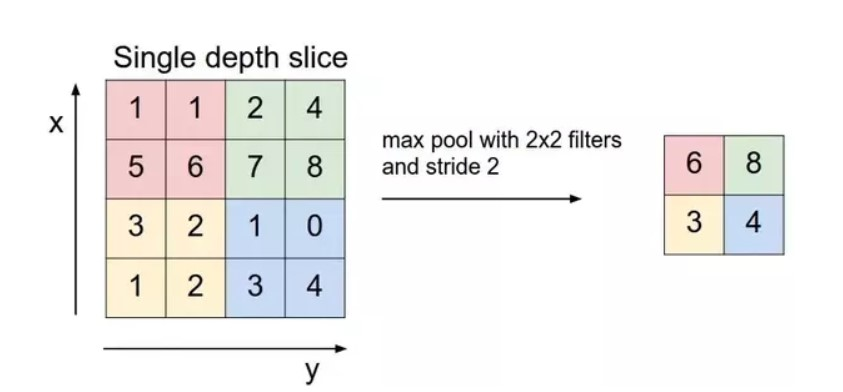
\includegraphics[scale=1]{Chapter2/max_pooling.jpg}	
	\caption{Max Pooling}
	\label{fig:maxpool}
\end{figure}
% INSERT MAX POOLING IMAGE HERE.

\subsection{Fully Connected Layer}
The input to the fully connected layer is the output from the final Pooling or Convolutional Layer, which is flattened (unroll the output of final (and any) Pooling and Convolutional Layer, which is a 3-dimensional matrix, values into a vector) and then fed into the fully connected layer.

\begin{figure}[H]
\centering
	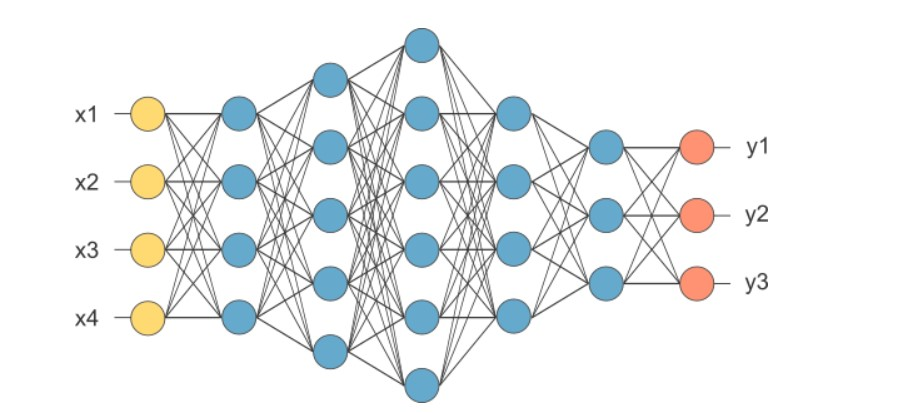
\includegraphics[scale=1]{Chapter2/after_pooling_layer_flattened_as_FC_layer.jpg}	
	\caption{After pooling layer, flattened as FC layer}
	\label{fig:after_pooling}
\end{figure}
% INSERT AFTERPOOLINGFLATTENED..FC IMAGE HERE.

In the above diagram, the feature map matrix will be converted as vector (x1, x2, x3, ...). With the Fully Connected Layers, we combine these features together to create a model. Finally, we have an activation function such as softmax or sigmoid to classify the outputs as  car, truck, cat, dog, etc.

\section{Other parameters associated with \acrshort{cnn} layers}

\subsection{Stride} 
It is the number of pixels shifts over the input matrix. We move the filter 1 pixel at a time when the stride is 1. We move the filter 2 pixels at a time when the stride is 2 and so on. Figure \ref{fig:stride} shows convolution would work with a stride of 2.

\begin{figure}[H]
\centering
	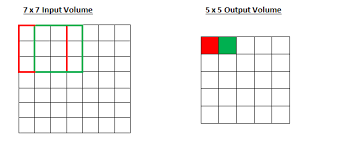
\includegraphics[scale=1]{Chapter2/stride.png}
	\caption{Stride}
	\label{fig:stride}
\end{figure}
% INSERT STRIDE IMAGE HERE.

\subsection{Padding}
There are times when the filter does not perfectly fit the input image. In such cases, there are two options:
\begin{enumerate}
    \item Pad the picture with zeros (zero-padding) so that it fits
    \item Drop the part of the image where the filter did not fit. This is called valid padding which keeps only valid part of the image.
\end{enumerate}

\subsection{Non Linear Activation function}
Activation functions are mathematical equations that determine the output of a neural network. The function is attached to each neuron in the network, and determines whether it should be activated (“fired”) or not, based on whether each neuron's input is relevant for the model's prediction. An example for activation function is ReLU (Rectified Linear Unit). ReLU is a non linear activation function defined as ƒ(x) $=$ max(0,x). It will output the input directly if it is positive, otherwise, it will output zero. It has become the default activation function for many types of neural networks since the problem of having negative weights can be avoided as negative values will be scaled to 0.

\begin{figure}[H]
\centering
	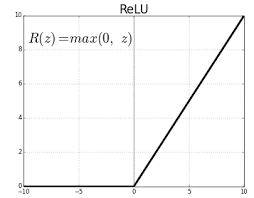
\includegraphics[scale=1]{Chapter2/relu.png}	
	\caption{ReLU activation Function}
	\label{fig:relu}
\end{figure}
% INSERT RELU IMAGE HERE.



% \section{Summary}
In summary, the CNN architecture is as follows. The input image is provided to the convolution layer. Parameters are chosen, filters with strides are applied along with padding, if required. Convolution on the image is performed and a non linear activation is applied to the matrix. Pooling is performed to reduce image dimension. The output of this stage is flattened and fed into a fully connected layer (FC Layer). This layer outputs the class to which the input image belongs.
\begin{figure}[H]
\centering
	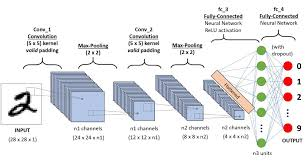
\includegraphics[scale=1.25]{Chapter2/cnn.jpeg}	
	\caption{CNN architecture}
	\label{fig:CNN}
\end{figure}
% INSERT COMPLETE CNN ARCHITECTURE IMAGE HERE.


%Chapter 3
\chapter{Design of Pipelined Analog to Digital converter}

\indent\indent Every chapter should start with an introduction paragraph. This paragraph should brief about the flow of the chapter. This introduction can be limited within 4 to 5 sentences. The chapter heading should be appropriately modified (a sample heading is shown for this chapter). 
\section{Contents of this Chapter}
This chapter should contain the following sections and subsections in detail.
\begin{enumerate}
\item Specifications for the Design
\item Pre analysis work for the design or Models used
\item Design methodology in detail
\item Design Equations
\item Experimental techniques (if any)
\end{enumerate}
Apart from the aforementioned sections, you can add sections as per the requirements of the project in consultation with your guide.

\section{Paraphrasing}
When you paraphrase a written passage, you rewrite it to state the essential ideas in your own words. Because you do not quote your source word for word when paraphrasing, it is unnecessary to enclose the paraphrased material in quotation marks. However, the paraphrased material must be properly referenced because the ideas are taken from someone else whether or not the words are identical. 

Ordinarily, the majority of the notes you take during the research phase of writing your report will paraphrase the original material. Paraphrase only the essential ideas. Strive to put original ideas into your own words without distorting them."

\section{Quotations}
When you have borrowed words, facts, or idea of any kind from someone else's work, acknowledge your debt by giving your source credit in footnote (or in running text as cited reference). Otherwise, you will be guilty of plagiarism. Also, be sure you have represented the original material honestly and accurately. Direct word to word quotations are enclosed in quotation marks."

\vspace{0.75cm}

After elaborating the various sections of the chapter, a summary paragraph should be written discussing the highlights of that particular chapter. This summary paragraph should not be numbered separately.  

%Chapter 4
\chapter{Implementation of Pipelined Analog to Digital converter}

\indent\indent Every chapter should start with an introduction paragraph. This paragraph should brief about the flow of the chapter. This introduction can be limited within 4 to 5 sentences. The chapter heading should be appropriately modified (a sample heading is shown for this chapter). 

\section{Contents of this chapter}
This chapter should elaborate the following in detail.
\begin{enumerate}
\item Implementation details for hardware based projects
\item Top level Design for software based projects
\end{enumerate}

You can add sections and sub sections to elaborate your project work done.

\vspace{0.75cm}

After elaborating the various sections of the chapter, a summary paragraph should be written discussing the highlights of that particular chapter. This summary paragraph should not be numbered separately.  



%Chapter 5
\chapter{Results \& Discussions}
\indent\indent Every chapter should start with an introduction paragraph. This paragraph should brief about the flow of the chapter. This introduction can be limited within 4 to 5 sentences. The chapter heading should be appropriately modified (a sample heading is shown for this chapter). 
\section{Contents of this chapter}
All the results obtained for your objectives should be discussed in this chapter. This chapter should contain the following sections as per the project.
\begin{enumerate}
\item Simulation results
\item Experimental results
\item Performance Comparison
\item Inferences drawn from the results obtained
\end{enumerate}
All the figures should be properly explained by bringing the scenarios of the design done in the project. A detailed discussion of results obtained should be done in this chapter.

\section{Tables in thesis}
\begin{itemize}
	\item All Table Caption should be in Sentence Case, TNR 10 Pt. It should be of the Format:
	\begin{itemize}
		\item Table 1.1 Results of the experiment ….(Centered)
	\end{itemize}
	\item It should be cited as Table 1.1.
	\item Caption should appear above the Table.
	\item Table Header and the entries should be of Font TNR 10 Pt, Justified.
	\item For wider Table, the page orientation can be Landscape.
	\item For Larger Table, it can run to pages and the header should be repeated for each page of the Table.
	\item Table must be adjusted to fit in the page and no single row is left out for a new page.	
\end{itemize}

Sample Table \ref{c5:tab1} and Table \ref{c5:tab2} are given below  for your reference,

\begin{table}[htb]
\fontsize{10}{12}\selectfont
\caption{Country List}
\label{c5:tab1}
\begin{tabular}{|p{3cm}|c|c|c|}
	%\hline
	%\multicolumn{4}{|c|}{Country List} \\
	\hline
	\textbf{Country Name     or Area Name}& \textbf {ISO ALPHA 2 Code} & \textbf {ISO ALPHA 3 Code} & \textbf{ISO numeric Code}\\
	\hline
	\textbf{Afghanistan}   & AF    & AFG &   004\\\hline
	\textbf{Aland Islands}&   AX  & ALA   & 248\\\hline
	\textbf{Albania} & AL & ALB&  008\\\hline
	\textbf{Algeria}    &DZ & DZA&  012\\\hline
	\textbf{American Samoa}&   AS  & ASM&016\\\hline
	\textbf{Andorra}& AD  & AND   & 020\\\hline
	\textbf{Angola}& AO  & AGO& 024\\
	\hline
\end{tabular}
\end{table}

%\begin{table}[htp]
%\fontsize{10}{12}\selectfont
%\centering
%\caption{Data units, sources, and dates} \label{c5:tab2}
%\begin{tabular}{| *4{>{\arraybackslash}m{1in}|} @{}m{0pt}@{}}
%	\hline
%	\textbf{Variable} & \textbf{Dates} & \textbf{Units} &
%	\textbf{Source}  &\\[2ex] 
%	\hline
%	\textbf{Nominal Physical Capital Stock} & 1950-1990 & Billions
%			US\$ & Nehru and Dhareshwar (1993) &\\[0ex]
%	\hline
%	\textbf{Total Population} & 1950-1990 & Billions & Nehru and
%			Dhareshwar (1993) &\\[0ex]
%	\hline
%	\textbf{Nominal GDP} & 1950-1990 & Billions  US\$ & PWT &\\[5ex]
%	\hline
%	\textbf{Real GDP per capita} & 1950-1990 & 2005 US\$ per capita & PWT &\\[5ex]
%	\hline
%\end{tabular}
%\end{table}

\section{Math equation in thesis}
All equation should be written using equation editor or using an equivalent tool.
\begin{itemize}
	\item Equations should be numbered as : 1.1, 1.2 ...
	\item Equation should be Centered, 12 Pt, TNR. 
	\item Equation number should be right Justified
	\item It should be cited as Eqn. 1.1.
   \item If the sentence starts by citing an equation, then it should be written as Equation 1.1 For example, Equation 5.1 states the Pythagoras theorem.

	
\end{itemize}

For example in Eqn. \ref{c5:eqn1}, The well known Pythagorean theorem $x^2 + y^2 = z^2$ was 
proved to be invalid for other exponents. 
Meaning the next equation has no integer solutions:

\begin{equation}
\label{c5:eqn1}
	x^n + y^n = z^n
\end{equation}

The mass-energy equivalence is described by the famous equation in Eqn. \ref{c5:eqn2}
\begin{equation}
\label{c5:eqn2}
	E=mc^2
\end{equation}

discovered in 1905 by Albert Einstein. 

\vspace{0.75cm}

After elaborating the various sections of the chapter, a summary paragraph should be written discussing the highlights of that particular chapter. This summary paragraph should not be numbered separately.  






%Chapter 6
\chapter{Conclusion and Future Scope}

\section{Conclusion}
This chapter should not contain an introduction paragraph like other chapters. You can directly write conclusion of the work done under this section. Typically this section can have 3 to 4 paragraphs. 

First paragraph should bring in the scenario of the project and every objective should be explained here.

Second paragraph should say how the objectives are implemented and achieved.

Last paragraph should draw the conclusions from each objective with quantitative results, performance improvement etc. 

\section{Future Scope}
Briefly discuss the constraints and limitations of the project and state the possibilities of extending the work in future.
\section{Learning Outcomes of the Project}
\begin{itemize}
\item List the learning outcomes here
\item List a minimum of 5 learning outcomes
\end{itemize}



\backmatter
\clearpage
%\ifDrft{
%%Do Nothing
%}\else{
\printbibliography%
%}
%\printindex
\end{spacing}
\end{document}